\documentclass{beamer}

\mode<presentation>
{
	\usetheme{CambridgeUS}
	\usecolortheme{orchid}
	\setbeamercovered{transparent}
	\useinnertheme{rectangles}
	\setbeamertemplate{navigation symbols}{}
	\usefonttheme[onlymath]{serif}
	\setbeamercolor{title}{bg=alerted text.fg!85!black, fg=white}
	\setbeamercolor{item projected}{bg=alerted text.fg!85!black}
	\setbeamertemplate{enumerate items}[default]
	\setbeamercolor{local structure}{fg=alerted text.fg!85!black}
}

\usepackage[english]{babel}
\usepackage[utf8]{inputenc}
\usepackage[T1]{fontenc}
\usepackage{lmodern}
\usepackage{pifont}
\usepackage{mathrsfs}
\usepackage{amsmath}
\usepackage{bm}
\usepackage{caption}
\usepackage{subcaption}
\usepackage{outlines}
\usepackage{booktabs}
\usepackage[%
	autocite     = plain,
	doi          = true,
	url          = true,
	giveninits   = true,
	hyperref     = true,
	backref      = true,
	maxbibnames  = 99,
	maxcitenames = 99,
	sortcites    = true,
	style        = authoryear,
]{biblatex}

% \input{bibliography-mimosis}
\addbibresource{presentation.bib}

\newcommand{\fakeimage}{{\fboxsep=-\fboxrule\fbox{\rule{0pt}{3cm}\hspace{4cm}}}}

\usepackage{tikz}
\usetikzlibrary{bayesnet}
\usetikzlibrary{arrows,calc,positioning,decorations.pathreplacing}
\tikzset{
	>=stealth',
	punkt/.style={
			circle,
			draw=black, thick,
			minimum height=1.75em,
			inner sep=0pt,
			text centered},
	pil/.style={
			->,
			thick}
}
\definecolor{hdblue}{HTML}{3366cc}
\hypersetup{colorlinks,linkcolor=,urlcolor=hdblue, citecolor=hdblue}


\newcommand{\xmark}{\ding{55}}
\newcommand{\highlight}[1]{%
	\colorbox{red!50}{$\displaystyle#1$}}


\def\ci{\perp\!\!\!\perp}
\makeatletter
\newcommand*{\indep}{%
	\mathbin{%
		\mathpalette{\@indep}{}%
	}%
}
\newcommand*{\nindep}{%
	\mathbin{%                   % The final symbol is a binary math operator
		\mathpalette{\@indep}{\not}% \mathpalette helps for the adaptation
		% of the symbol to the different math styles.
	}%
}
\def\layersep{.38cm}
\def\inlsep{.4}
\newcommand*{\@indep}[2]{%
	% #1: math style
	% #2: empty or \not
	\sbox0{$#1\perp\m@th$}%        box 0 contains \perp symbol
	\sbox2{$#1=$}%                 box 2 for the height of =
	\sbox4{$#1\vcenter{}$}%        box 4 for the height of the math axis
	\rlap{\copy0}%                 first \perp
	\dimen@=\dimexpr\ht2-\ht4-.2pt\relax
	% The equals symbol is centered around the math axis.
	% The following equations are used to calculate the
	% right shift of the second \perp:
	% [1] ht(equals) - ht(math_axis) = line_width + 0.5 gap
	% [2] right_shift(second_perp) = line_width + gap
	% The line width is approximated by the default line width of 0.4pt
	\kern\dimen@
	{#2}%
	% {\not} in case of \nindep;
	% the braces convert the relational symbol \not to an ordinary
	% math object without additional horizontal spacing.
	\kern\dimen@
	\copy0 %                       second \perp
}
\makeatother


\title[CGNN]{Learning Functional Causal Models with Generative Neural Networks}

% \subtitle
% {Presentation Subtitle} % (optional)

\author[Dogan]
{%
	\texorpdfstring{
		\begin{columns}
			\column{.45\linewidth}
			\centering
			Presented by:\\
			Haluk Dogan\\
			\url{https://haluk.github.io/}\\
			\href{mailto:hdogan@vivaldi.net}{hdogan@vivaldi.net}
		\end{columns}
	}
	{Dogan}
}
\institute[UNL] % (optional, but mostly needed)
{
	Department of Computer Science\\
	University of Nebraska-Lincoln
}

\date[\today] % (optional)
{\today}

\subject{Talks}

\pgfdeclareimage[height=0.5cm]{university-logo}{img/logo}
\logo{\pgfuseimage{university-logo}}

% Delete this, if you do not want the table of contents to pop up at
% the beginning of each subsection:
\AtBeginSubsection[]
{
	\begin{frame}<beamer>{Outline}
		\tableofcontents[currentsection,currentsubsection]
	\end{frame}
}

%\tikzset{every picture/.style={line width=0.75pt}}

\begin{document}

\begin{frame}
	\titlepage{}
\end{frame}

\section{Introduction}
\begin{frame}{Introduction}
	\begin{columns}
		\begin{column}{.48\textwidth}
			\begin{figure}[ht]
				\centering
				\input{img/weatherbn.tikz}
				\caption*{\tiny{C:\@ Cloudy, R:\@ Rainy, S:\@ Sprinkler, W:\@ WetGrass}\label{fig:weather-bn}}
			\end{figure}
			\vspace{-0.5cm}
			\begin{figure}[ht]
				\centering
				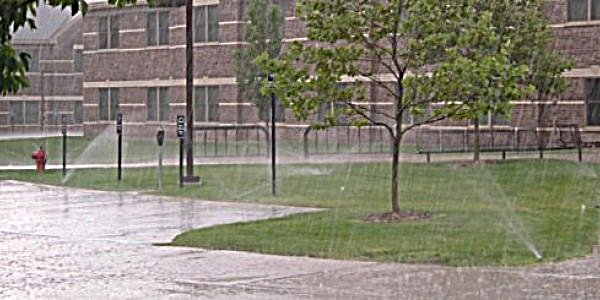
\includegraphics[width=1\textwidth, keepaspectratio]{img/sprinklerrain.jpg}
				\caption*{\label{fig:sprinkler-rain}}
			\end{figure}
		\end{column}
		\begin{column}{.48\textwidth}
			\begin{align*}
				R, E_{S}, E_{W} & \leftarrow U(0,1)       \\
				S               & \leftarrow 0.5R + E_{S} \\
				W               & \leftarrow S + E_{W}
			\end{align*}
			\begin{center}
				\tikz{ %
					\node[obs] (R) {$R$};
					\node[obs, right=of R] (S) {$S$};
					\node[obs, right=of S] (W) {$W$};
					\edge {R} {S};
					\edge {S} {W};
				}
			\end{center}
			\vspace{-0.5cm}
			\tiny{
				\begin{block}{Regression Solution}
					\[
						\hat{S} = 0.25R + 0.5W
					\]
				\end{block}
				\begin{block}{Derivation}
					$S = B_{1}R + B_{2}W$\\
					$S = 0.5R+E_{S}=W-E_{W}$ \\
					$E_{S} \sim E_{W}$ so $S \sim W$ \\
					$S=0.5 \times U(0,1) + U(0,1)$ \\
					\vspace{-0.5cm}
					\begin{align*}
						E(S \mid R, W) & = 0.5 \times E_{R} \times R + E_{W} \times W \\
						               & = 0.25R + 0.5W
					\end{align*}
				\end{block}
			}
		\end{column}
	\end{columns}
\end{frame}

\begin{frame}{Introduction (cont'd)}
	\begin{columns}
		\begin{column}{.38\textwidth}
			\begin{figure}[ht]
				\centering
				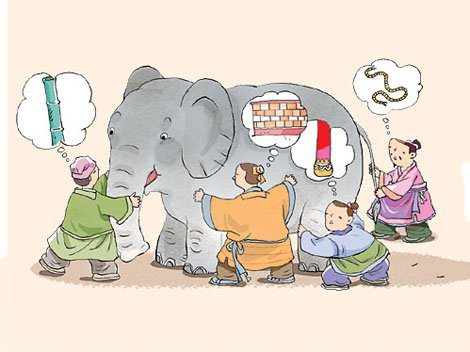
\includegraphics[width=1\textwidth, keepaspectratio]{img/elephant.jpg}
			\end{figure}
			\vspace{-0.5cm}
			\begin{figure}[ht]
				\centering
				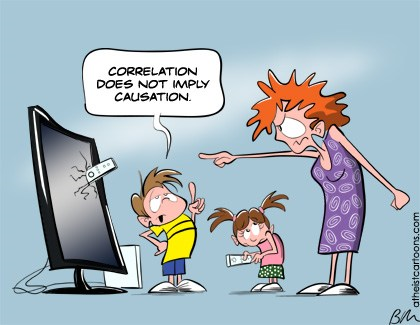
\includegraphics[width=1\textwidth, keepaspectratio]{img/correlation_causation.png}
			\end{figure}
		\end{column}
		\begin{column}{.58\textwidth}

			\begin{figure}[ht]
				\centering
				\scalebox{0.6}{\input{img/asia.tikz}}
			\end{figure}
			\vspace{-0.8cm}
			\begin{flalign*}
				P(X_{1},&\dots,X_{8}) = P(X_{1})P(X_{2})P(X_{3} \mid X_{1}) &\\
				& P(X_{4} \mid X_{2})P(X_{5} \mid X_{2})P(X_{6} \mid X_{3},X_{4})&\\
				&P(X_{7} \mid X_{6})P(X_{8} \mid X_{5},X_{6})
			\end{flalign*}
			Assuming variables are boolean: \\
			\textbf{Representation cost:}
			\begin{itemize}
				\item Joint probability: $2^{8}$
				\item BN:\@ $2+2+4+4+4+8+4+8=36$
			\end{itemize}
		\end{column}
	\end{columns}
\end{frame}

\begin{frame}{Introduction (cont'd)}
	\begin{block}{Marginal Independence}
		$X \ci Y$ iff
		\begin{flalign*}
			& P(X,Y)      = P(X)P(Y) &\\
			& P(X \mid Y) = P(X)     &\\
			& P(Y \mid X) = P(Y)&
		\end{flalign*}
	\end{block}
	\begin{block}{Conditional Independence}
		$P(X \ci Y \mid Z)$ iff
		\begin{flalign*}
			& P(X,Y \mid Z) = P(X \mid Z) P(Y \mid Z) &\\
			& P(X \mid Y,Z) = P(X \mid Z) &\\
			& P(Y \mid X,Z) = P(Y \mid Z)
		\end{flalign*}
	\end{block}
\end{frame}
\begin{frame}{Introduction (cont'd)}
	Discovering causal relations requires performing experiments
	\begin{itemize}
		\item unethical
		\item expensive
		\item difficult to repeat
	\end{itemize}
	\begin{block}{Interventation}
		$\bm{X} = [X_{1},\dots,X_{d}]$\\
		$do(X_{i}=x)$
	\end{block}
	\begin{block}{Direct Cause}
		$X_{i} \rightarrow X_{j}$ iff \\
		$P(X_{j} \mid do(X_{i}=x,\bm{X}_{\setminus ij}=\bm{c})) \neq P(X_{j} \mid do(X_{i}=x',\bm{X}_{\setminus ij}=\bm{c}))$
	\end{block}

\end{frame}

\begin{frame}{Outline}
	\tableofcontents
\end{frame}

\begin{frame}{Functional Causal Model (FCM)}
	\begin{figure}[ht]
		\centering
		\scalebox{0.7}{\input{img/FCM.tikz}}
		\caption*{\label{fig:FCM} }
	\end{figure}
	\vspace{-1cm}
	\begin{itemize}
		\item FCM on a random variable vector $\bm{X}=[X_{1},\dots,X_{d}]$ is a triplet $(\mathscr{G}, f, \mathscr{E})$
		\item $X_{i} \leftarrow f_{i}(X_{{\text{Pa}(i;\mathscr{G})}}, E_{i})$, $E_{i} \sim \mathscr{E}$, for $i=1,\dots,d$
		\item $E_{i}$ is used to account all unobserved variables and noise
	\end{itemize}
\end{frame}

\begin{frame}{Assumptions and Properties}
	\begin{itemize}
		\item Causal sufficiency assumption (\textbf{CSA}): common causes of all variables are measured\\ \vspace{0.2cm}
		      \begin{columns}
			      \begin{column}{.30\textwidth}
				      \tikz{
					      \node[latent] (A) {\texttt{A}};
					      \node[obs, below left=of A] (SS) {\texttt{SS}};
					      \node[obs, below right=of A] (IQ) {\texttt{IQ}};
					      \edge {A} {SS, IQ};
				      }
			      \end{column}

			      \begin{column}{.58\textwidth}
				      \begin{itemize}
					      \item \texttt{SS} $\ci$ \texttt{IQ} $\mid$ \texttt{A}
					      \item Suppose \texttt{A} is unmeasured
					      \item Data will only include independence statements not conditioned on \texttt{A}
				      \end{itemize}

			      \end{column}
		      \end{columns}
	\end{itemize}
\end{frame}
\begin{frame}{Assumptions and Properties (cont'd)}
	\begin{itemize}
		\item Causal Markov assumption (\textbf{CMA}):\\
		      r.v $\ci$ non-descendants (non-effects) $\mid$ parents (direct causes) by~\cite{Spirtes2001}
		\item For an FCM, this assumption holds if the graph is a DAG and error terms $E_{i}$ in the FCM are independent on each other
		      \begin{figure}[ht]
			      \centering
			      \scalebox{0.7}{\input{img/FCM_Pearl.tikz}}
			      \caption*{\label{fig:FCM-Pearl} }
		      \end{figure}

	\end{itemize}
\end{frame}
\begin{frame}{Assumptions and Properties (cont'd)}
	\begin{itemize}
		\item Conditional independence relations in an FCM:\\
		      If \textbf{CMA} applies, the data generated by the FCM satisfy all CI relations in $\bm{X}$ via d-separation by~\cite{Pearl2009}
	\end{itemize}
	\begin{alertblock}{Faithfulness Assumption}
		There may be more CIs in data than present in the model
	\end{alertblock}
\end{frame}
\begin{frame}{Assumptions and Properties (cond't)}
	\begin{columns}
		\begin{column}{.48\textwidth}
			\begin{figure}[ht]
				\centering
				\input{img/faithfulness1.tikz}
			\end{figure}
		\end{column}
		\begin{column}{.48\textwidth}
			\begin{figure}[ht]
				\centering
				\input{img/faithfulness2.tikz}
			\end{figure}
		\end{column}
	\end{columns}
	\scalebox{0.8}{
		\begin{columns}
			\begin{column}{.48\textwidth}
				\begin{flalign*}
					&a \times c + b =0, E_{\bm{\cdot}} \sim N(0, \sigma_{{\bm{\cdot}}}^{2}) &\\
					&X = E_{x} &\\
					&Y = aX+E_{Y} &\\
					&Z = bX + cY + E_{Z} &\\
					&Z = -acX + c(aX+E_{Y})+E_{Z}&\\
					&Z = cE_{Y} + E_{Z}
				\end{flalign*}
			\end{column}\hspace{1cm}
			\begin{column}{.48\textwidth}
				\begin{flalign*}
					&\tilde{a}=a, \tilde{b}= (b\sigma_{Y}^{2})/(b^{2}\sigma_{Y}^{2}+\sigma_{Z}^{2}), E_{\bm{\cdot}} \sim N(0, \tau_{{\bm{\cdot}}}^{2}) &\\
					&\tau_{X}^{2}=\sigma_{X}^{2} &\\
					&\tau_{Y}^{2}=\sigma_{Y}^{2}-(b^{2}\sigma_{Y}^{4})/(b^{2}\sigma_{Y}^{2}+\sigma_{Z}^{2})&\\
					&\tau_{Z}^{2}=b^{2}\sigma_{Y}^{2}+\sigma_{Z}^{2} &\\
					&\Sigma=\left(\begin{array}{ccc}{\sigma_{X}^{2}} & {a \sigma_{X}^{2}} & {0} \\ {a \sigma_{X}^{2}} & {a^{2} \sigma_{X}^{2}+\sigma_{Y}^{2}} & {b \sigma_{Y}^{2}} \\ {0} & {b \sigma_{Y}^{2}} & {b^{2} \sigma_{Y}^{2}+\sigma_{Z}^{2}}\end{array}\right) &\\
				\end{flalign*}
			\end{column}
		\end{columns}
	}
\end{frame}
\begin{frame}{Assumptions and Properties (cont'd)}
	\begin{itemize}
		\item v-structure property: $(X \nindep Z \mid Y)$\\\vspace{1cm}
		      \tikz{
			      \node[obs] (X) {$X$};
			      \node[obs, below right=of X] (Y) {$Y$};
			      \node[obs, above right=of Y] (Z) {$Z$};
			      \edge{X,Z} {Y};
		      }

	\end{itemize}
\end{frame}

\section{Structure Learning}
\begin{frame}{Learning the CPDAG}
	\begin{figure}
		\begin{subfigure}{.30\linewidth}
			\scalebox{0.9}{\input{img/skeleton.tikz}}
			\caption{Skeleton of a DAG}\label{fig:skeleton-dag}
		\end{subfigure}
		\hfill
		\begin{subfigure}{.30\linewidth}
			\scalebox{0.9}{\input{img/exactdag.tikz}}
			\caption{Exact DAG}\label{fig:exact-dag}
		\end{subfigure}
		\hfill
		\begin{subfigure}{0.30\linewidth}
			\scalebox{0.9}{\input{img/markoveq2.tikz}}
			\caption{Markov equivalent DAG}\label{fig:markov2}
		\end{subfigure}
		\bigskip
		\begin{subfigure}{0.45\linewidth}
			\scalebox{0.9}{\input{img/markoveq1.tikz}}
			\caption{Markov equivalent DAG}\label{fig:markov1}
		\end{subfigure}
		\hfill
		\begin{subfigure}{.45\linewidth}
			\scalebox{0.9}{\input{img/cpdag.tikz}}
			\caption{CPDAG}\label{fig:cpdag}
		\end{subfigure}
	\end{figure}
\end{frame}
\begin{frame}{Learning Algorithms}
	\begin{itemize}
		\item \textbf{Constraint based}: Recover graph structure using tests of conditional independence
		\item \textbf{Score based}: Explore space of graphs while maximizing some scoring function defined relative to data
		\item \textbf{Hybrid}: Combination of constraint / score based methods
		\item \textbf{Pairwise}:
		      \begin{itemize}
			      \item Restricting the class of functions allowed for causal mechanisms $f_{i}$ and assuming a functional form
			      \item Regularize functions $f_{i}$ with respect to local score and (empirically) helps the problem of identifiability
		      \end{itemize}
	\end{itemize}
\end{frame}
\section{FCGNN}
\begin{frame}{FCGNN}
	\begin{figure}[ht]
		\centering
		\scalebox{0.9}{\input{img/FCGNN.tikz}}
		\caption*{\label{fig:FCGNN-arch} }
	\end{figure}
	\vspace{-1cm}
	\[\hat{X}_i  =  \hat{f}_i(\hat{X}_{\text{Pa}(i;\mathscr{G})}, E_i)
		=  \sum_{k=1}^{n_h} \bar{w}^{i}_k \sigma \left(\sum_{j \in \text{Pa}(i;\mathscr{G})} \hat{w}^{i}_{jk} \hat{X}_j
		+ w^{i}_{k} E_i +  b^{i}_k \right) +\bar{b}^{i}
	\]
\end{frame}
\begin{frame}{FCGNN (cont'd)}
	\[
		S(\mathscr{C}_{\hat{\mathscr{G}},\hat{f}}, \mathscr{D}) =
		\widehat{\text{MMD}}_k(\mathscr{D}, \widehat{\mathscr{D}}) + \lambda
		|\widehat{\mathscr{G}}|
	\]
	\[
		\widehat{\text{MMD}_k}(\mathscr{D}, \widehat{\mathscr{D}}) =
		\frac{1}{n^2} \sum_{i, j = 1}^{n} k(x_i, x_j) +
		\frac{1}{n^2} \sum_{i, j = 1}^{n} k(\hat{x}_i, \hat{x}_j)
		- \frac{2}{n^2} \sum_{i,j = 1}^n k(x_i, \hat{x}_j)
	\]
	\begin{itemize}
		\item $k$: Gaussian kernel, $k(x,x') = \exp(-\gamma \|x-x'\|_2^2)$, differentiable
		\item $\lambda|\widehat{\mathscr{G}}|$ is a penalty term used for fair comparisons
	\end{itemize}
\end{frame}
\begin{frame}{Weight Optimization}
	\[
		\min _{ \hat{\mathscr{G} }_{ i } }{ \widehat{\text{MMD}}_{k}(\mathscr{D}, (\hat{\mathscr{G}_{i}}, \hat{f}_{1} \dots \hat{f}_{d}, \mathscr{E})) }
	\]
	\begin{itemize}
		\item Adam optimizer
		\item Noise samples are drawn in each epoch (training and testing)
	\end{itemize}
\end{frame}
\begin{frame}{Structure Optimization}
	\begin{itemize}
		\item Number of DAGs are super-exponential in size $|V|$~\parencite{Robinson1977}
		      \begin{itemize}
			      \item Structure optimization intractable
		      \end{itemize}
		\item Initial graph skeleton recovered by other methods such as feature selection~\parencite{Yamada2014}
		      \begin{itemize}
			      \item optimizing the edge orientations
			      \item Compare $S(\mathscr{C}_{X_i \rightarrow X_j,\hat{f}}, \mathscr{D}_{ij})$ and $S(\mathscr{C}_{X_j \rightarrow X_i,\hat{f}}, \mathscr{D}_{ij})$
			      \item keep the one gives the smaller score
			      \item Complexity $O(|E|)$
		      \end{itemize}
		\item Remove cycles from an initial graph
		\item Hill-Climbing (local search minimization)
		      \[
			      S_{X_i \rightarrow X_j} = S(\mathscr{C}_{\hat{\mathcal{G}} - \{X_i \rightarrow X_j\},\hat{f}}, \mathscr{D}) - S(\mathscr{C}_{\hat{\cal G},\hat{f}}, \mathscr{D})
		      \]
	\end{itemize}
\end{frame}
\section{Experiments}
\begin{frame}{Bivariate and Multivariate Causal Structures}
	\begin{itemize}
		\item Bivariate: 1500 samples
		\item \textbf{CE-Cha}: 300 continuous variable pairs
		\item \textbf{CE-Net}: 300 pairs generated with NN (random cause, e.g., exponential, gamma, lognormal, laplace)
		\item \textbf{CE-Gauss}: 300 pairs $Y = f_{Y}(X,E_{Y}), X=f_{X}(E_{X})$
		\item \textbf{CE-Multi}: 300 artificial pairs (linear and polynomial)
		      \begin{itemize}
			      \item post additive noise: $Y=f(X)+E$
			      \item post multiplicative noise: $Y=f(X) \times E$
			      \item pre-additive noise: $Y=f(X+E)$
			      \item pre-multiplicative noise $Y=f(X \times E)$
		      \end{itemize}
		\item \textbf{CE-Tueb}: 99 real-world cause-effect pairs
		\item Multivariate: 500 samples, 20 variables
	\end{itemize}
\end{frame}
\begin{frame}{Bivariate and Multivariate Causal Structures (cont'd)}
	Bivariate:
	\begin{figure}[ht]
		\centering
		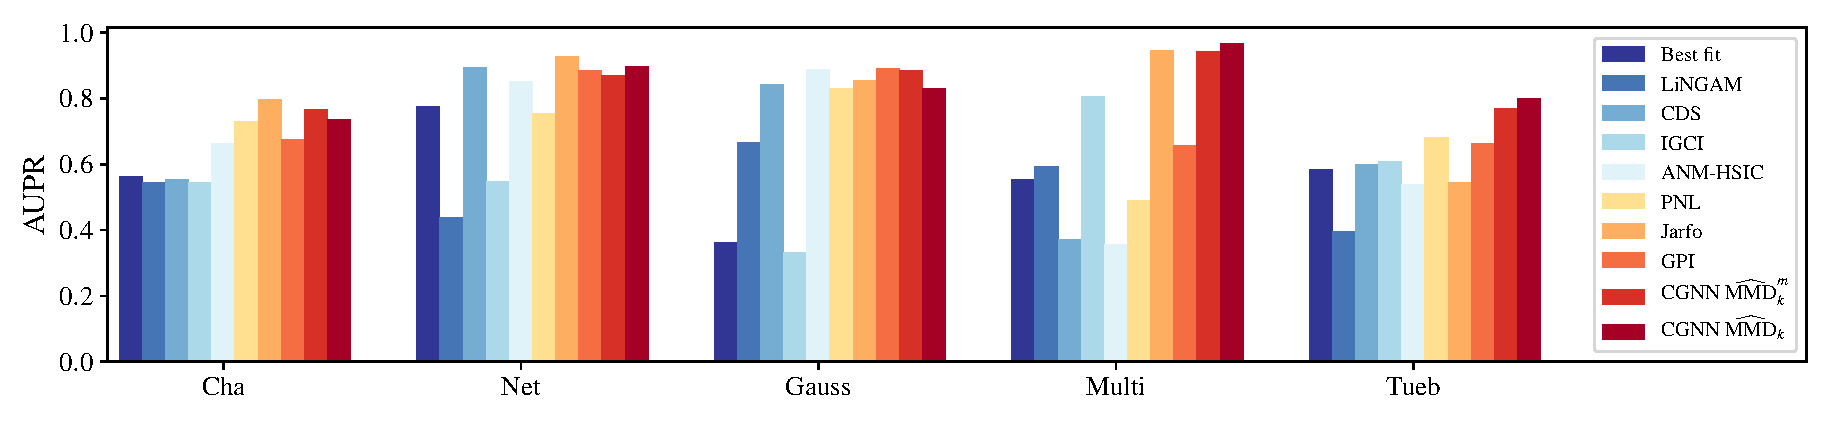
\includegraphics[width=1\textwidth,keepaspectratio]{img/aupr_pairwise.pdf}
		\caption*{\label{fig:auc-pairwise} }
	\end{figure}
	\vspace{-1cm}
	Multivariate:
	\begin{figure}[ht]
		\centering
		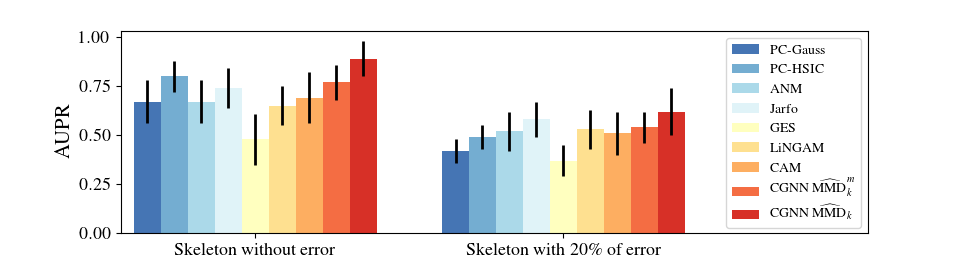
\includegraphics[width=0.95\textwidth,keepaspectratio]{img/graph_scores_multadd.png}
		\caption*{\label{fig:auc-multivariate} }
	\end{figure}

\end{frame}
\begin{frame}{Identifying v-Structures}
	500 samples
	\begin{figure}
		\begin{subfigure}{.24\linewidth}
			\scalebox{0.8}{\input{img/v-skel.tikz}}
			\caption{skeleton}\label{fig:skeleton-v}
		\end{subfigure}
		\hfill
		\begin{subfigure}{.24\linewidth}
			\scalebox{0.8}{\input{img/v-chain.tikz}}
			\caption{chain}\label{fig:chain-v}
		\end{subfigure}
		\hfill
		\begin{subfigure}{.24\linewidth}
			\scalebox{0.8}{\input{img/v-reverse.tikz}}
			\caption{reversed}\label{fig:rev-v}
		\end{subfigure}
		\hfill
		\begin{subfigure}{.24\linewidth}
			\scalebox{0.8}{\input{img/v.tikz}}
			\caption{v-structure}\label{fig:v}
		\end{subfigure}
	\end{figure}
	\begin{table}[!h]
		\label{table:acc_graph}
		\centering
		\begin{tabular}{l|cc|ccc}
			\toprule

			                       & \multicolumn{2}{c|}{non V-structures} & V structure \\
			Score                  & Chain str.                            &
			Reversed-V str.        & V-structure                                         \\
			\midrule
			$C_{ABC}$              & \textit{0.122 (0.009)}                &
			\textit{0.124 (0.007)} & 0.172 (0.005)                                       \\
			$C_{CBA}$              & \textit{0.121 (0.006)}                &
			\textit{0.127 (0.008)} & 0.171 (0.004)                                       \\
			$C_{reversed V}$       & \textit{0.122 (0.007)}                &
			\textit{0.125 (0.006)} & 0.172 (0.004)                                       \\ \hline
			$C_{Vstructure}$       & 0.202 (0.004)                         &
			0.180 (0.005)          & \textbf{0.127} (0.005)                              \\
		\end{tabular}
	\end{table}
\end{frame}

\section{Conclusion}
\begin{frame}{Questions}
	\begin{center}
		\Huge{Questions?}
	\end{center}
	\begin{figure}
		\centering
		
\includegraphics[width=0.5\textwidth, height=1.0\textheight, keepaspectratio]{img/walter.jpg}
	\end{figure}
\end{frame}
\begin{frame}[allowframebreaks]
	\frametitle{References}
	% \bibliographystyle{chicago}
	% \bibliography{presentation}
	\printbibliography{}
\end{frame}
\end{document}

%%% Local Variables:
%%% mode: latex
%%% TeX-master: t
%%% End:
